\chapter{ArchLinux installation}
\section{We are \textsc{Noobs}}
There are two ways to install ArchLinux on a Raspberry Pi: the first is 
the ArchLinux way -- no idea if it is the same with other systems -- and 
the second is an official manager which works with many systems.

\begin{itemize}
	\item follow instructions from archlinuxarm.org\footnote{Specific 
		  instruction on \href{http://archlinuxarm.org/platforms/armv6/
		  raspberry-pi}{archlinuxarm.org/platforms/armv6/raspberry-pi}} but 
		  you need to have a linux system
		  
	\item use \textsc{Noobs}, an operating system install manager provided by 
		  the Raspberry fundation\footnote{Details on \href{http://
		  www.raspberrypi.org/help/noobs-setup}{www.raspberrypi.org/help/
		  noobs-setup}}\\
\end{itemize}

I choose \textsc{Noobs} because it is the easiest way to install a
system on a RPi and in addition you get an extra \og{}boot manager\fg{} which 
is usefull. Moreover, you can complete the full setup of your SD card on any 
system by following the RPi website guide.
\\\\
\textsc{Noobs} is available on two forms: one for offline installation 
and the other -- the smallest one -- downloads automatically the last release 
of the system online. The offline installer contains many systems -- which 
takes a large space -- but you can just keep ArchLinux and remove others 
(in \texttt{os} folder). Anyway, you need to know that other systems files 
will be keeped after the installation so it is loose space. If you still want 
to use the offline way because you have no choices, you will have to find  
an older version of \textsc{Noobs} because ArchLinux has been removed since  
the last release.

\section{Installer usage}
According to the Noobs \href{http://www.raspberrypi.org/help/noobs-setup}
{documentation}, you just have to download the last Noobs release and format 
your SD card before unzip it and copy files on the card.
\\\\
After putting the card into the RPi and power on it, you will get the 
installer interface with a list of all systems you can install. If you choose 
the online way you have to connect your ethernet cable in the Raspberry even 
if you want to use a wifi dongle later.

\begin{figure}[h]
	\centering
	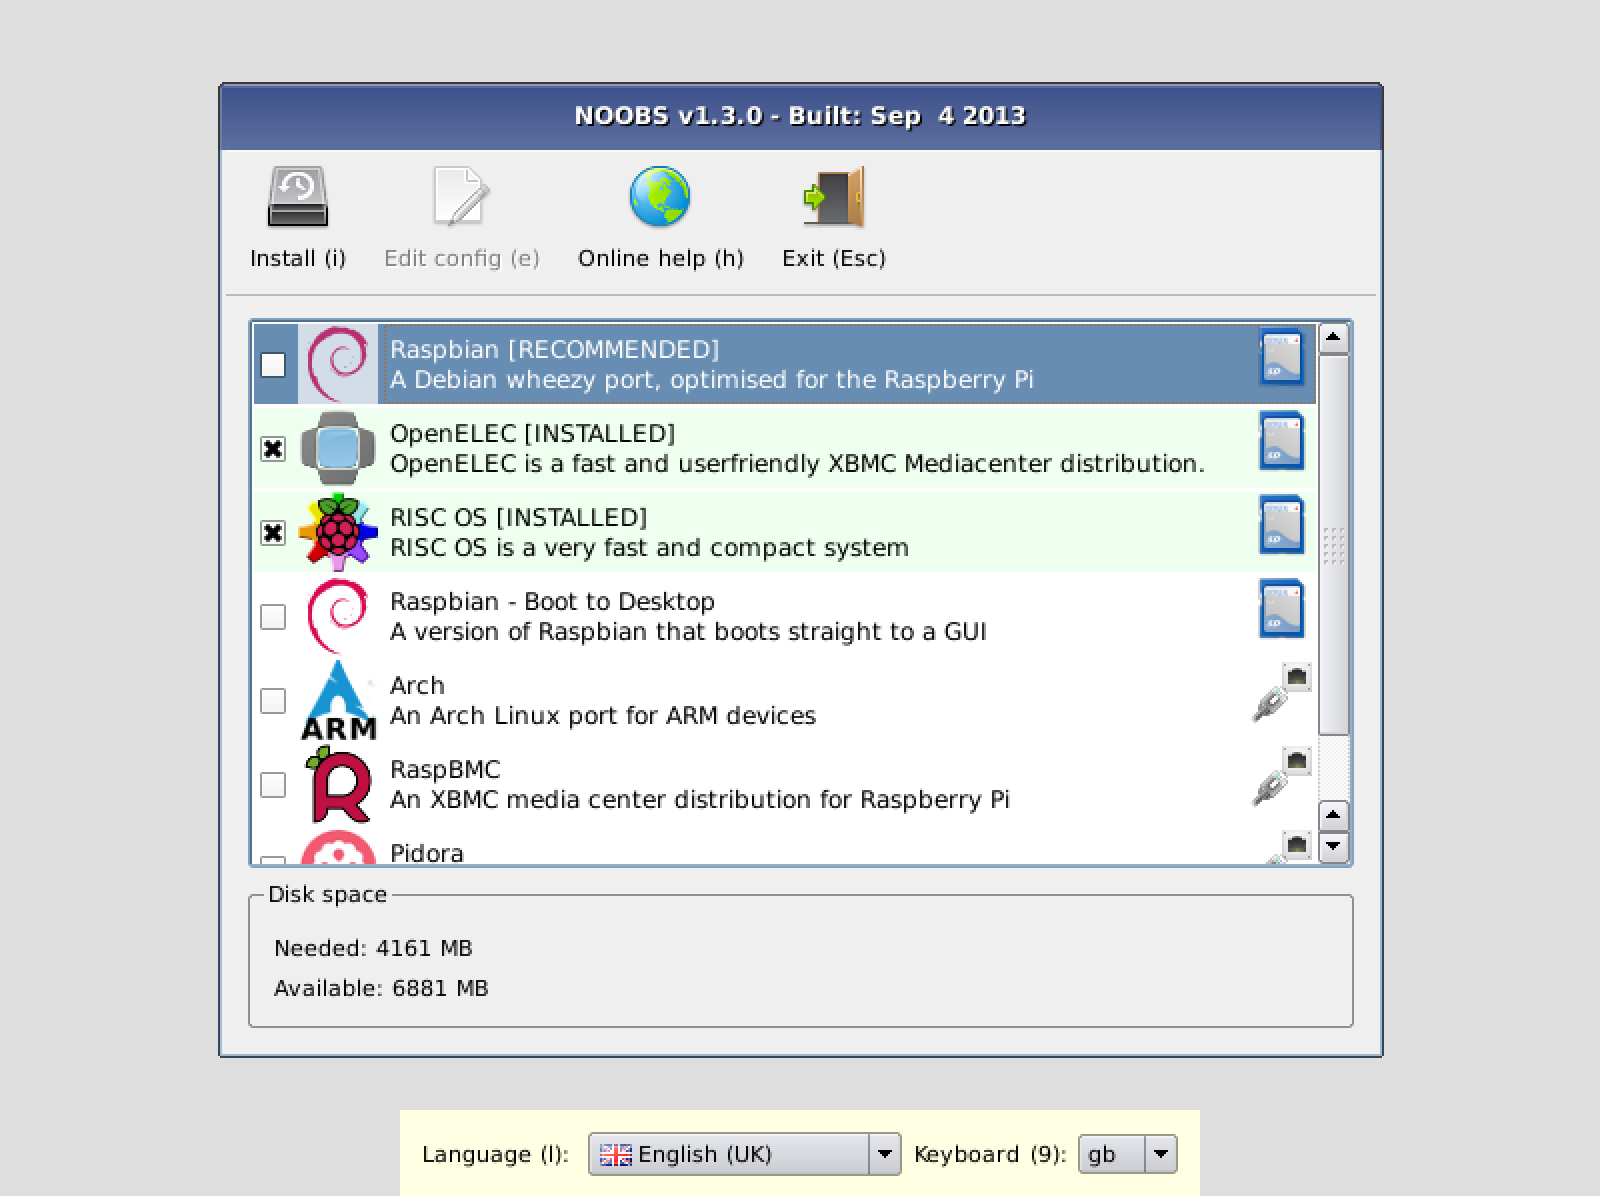
\includegraphics[scale=0.4]{images/NoobsMenu.png}
	\caption{Noobs installer menu}
	\label{figure:NoobsMenu}
\end{figure}

From the menu, select ArchLinux with arrow keys and press \og{}\texttt{space}
\fg{} to valid your choice. Then, you can change system and keyborad language with 
respectively \og{}\texttt{l}\fg{} and \og{}\texttt{0}\fg{} keys before 
pressing \og{}\texttt{i}\fg{} to begin ArchLinux installation on your RPi.
